\documentclass[a4paper]{article}
\usepackage[a4paper,margin=0mm]{geometry}
\usepackage{fontspec}
\usepackage{unicode-math}
\usepackage{tikz}
\usepackage[table]{xcolor}
\usepackage[absolute]{textpos}
\usepackage{enumitem}
\usepackage{array}
\usepackage{multirow}

\setmainfont{Libertinus Serif}
\setsansfont{Libertinus Sans}
\setmathfont{Libertinus Math}
\newfontfamily\trackedsans{Libertinus Sans}[LetterSpace=8.0]

\definecolor{accent}{HTML}{F46530}
\definecolor{badge}{HTML}{FFBDA5}
\definecolor{ink}{HTML}{2A2E30}

\setlength{\TPHorizModule}{1mm}
\setlength{\TPVertModule}{1mm}
\setlength{\parindent}{0pt}
\pagestyle{empty}

\newcommand{\LCOL}{16mm}
\newcommand{\RCOL}{111mm}
\newcommand{\COLW}{83mm}

\newcommand{\topicheader}[2]{%
\begin{textblock*}{194mm}(16mm,10mm)
\begin{tikzpicture}
\node[fill=accent,text=white,font=\sffamily\bfseries\fontsize{13}{13}\selectfont,
      minimum width=9mm,minimum height=9mm,inner sep=0pt] at (4.5mm,-4.5mm) {#1};
\node[font=\sffamily\bfseries\fontsize{15}{16}\selectfont,text=ink,anchor=west] at (12mm,-4.5mm) {#2};
\end{tikzpicture}
\end{textblock*}
\begin{textblock*}{194mm}(16mm,22.5mm)

\begin{tikzpicture}
\fill[accent] (0,0) rectangle (194mm,0.5mm);
\end{tikzpicture}
\end{textblock*}
}

\newcommand{\pagefooter}[1]{%
\begin{textblock*}{194mm}(8mm,286.41mm)
  
\begin{tikzpicture}
    \fill[accent] (0,0) rectangle (194mm,0.6mm);
  \end{tikzpicture}
\end{textblock*}
\begin{textblock*}{63.59mm}(8mm,288.27mm)
  {\sffamily\bfseries\color{accent}\fontsize{13}{16}\selectfont SAT 1200+}
\end{textblock*}
\begin{textblock*}{10mm}(188mm,288.27mm)
  \centering{\sffamily\color{accent}\fontsize{14}{16}\selectfont #1}
\end{textblock*}
}

\newcommand{\colrule}[2]{%
\begin{textblock*}{1mm}(105mm,#1mm)
\begin{tikzpicture}
\draw[black!65,line width=0.5pt] (0,0) -- (0,#2mm);
\end{tikzpicture}
\end{textblock*}
}

\newcommand{\setkicker}[2]{%
{\sffamily\bfseries\fontsize{12}{14}\selectfont #1.}\ {\itshape\fontsize{11}{14}\selectfont\color{black!75} #2}\par\vspace{2mm}%
}

\setlength{\fboxsep}{1.4pt}
\setlength{\fboxrule}{0.5pt}
\newcommand{\pnum}[1]{\fcolorbox{ink}{white}{\sffamily\bfseries\fontsize{8}{8}\selectfont #1}~}

\newcommand{\qrbox}[1]{%
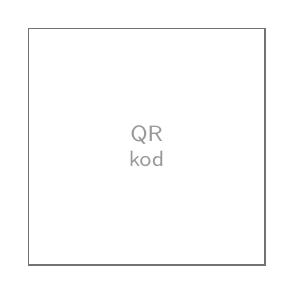
\begin{tikzpicture}
\draw[black!55,line width=0.6pt] (0,0) rectangle (30mm,30mm);
\node[black!40,font=\sffamily\fontsize{8}{9}\selectfont,align=center] at (15mm,15mm) {QR\\kod};
\end{tikzpicture}\\[1.5mm]
{\sffamily\fontsize{9}{11}\selectfont\color{black!70} #1}%
}

\arrayrulecolor{accent}
\setlength{\arrayrulewidth}{0.7pt}
\renewcommand{\arraystretch}{1.35}
\newcommand{\anstitle}[1]{{\sffamily\bfseries\color{accent}\fontsize{11}{13}\selectfont #1}\\[1.3mm]}

\begin{document}

% ================= PAGE 1: Set 1 | Set 2 =================
\topicheader{5}{Kvadrat tenglamalar I --- ko'paytuvchalash}
\pagefooter{1}
\colrule{32}{238}
\mbox{}%

\begin{textblock*}{\COLW}(\LCOL,32mm)
{\fontsize{12}{15}\selectfont
\setkicker{1-to'plam}{Ko'paytuvchalarga ajrating: $a=1$, $b$ va $c$ musbat.}

\noindent\pnum{1} $x^2+5x+4=0$\\[20mm]
\noindent\pnum{2} $x^2+6x+8=0$\\[20mm]
\noindent\pnum{3} $x^2+9x+14=0$\\[20mm]
\noindent\pnum{4} $x^2+3x+2=0$\\[20mm]
\noindent\pnum{5} $x^2+10x+16=0$\\[20mm]
\noindent\pnum{6} $x^2+8x+12=0$\\[20mm]
\noindent\pnum{7} $x^2+11x+18=0$\\[20mm]
\noindent\pnum{8} $x^2+7x+10=0$
}
\end{textblock*}

\begin{textblock*}{\COLW}(\RCOL,32mm)
{\fontsize{12}{15}\selectfont
\setkicker{2-to'plam}{Ko'paytuvchalarga ajrating: manfiy $b$ va/yoki $c$.}

\noindent\pnum{1} $x^2-5x+6=0$\\[20mm]
\noindent\pnum{2} $x^2+2x-15=0$\\[20mm]
\noindent\pnum{3} $x^2-3x-10=0$\\[20mm]
\noindent\pnum{4} $x^2-7x+12=0$\\[20mm]
\noindent\pnum{5} $x^2+4x-21=0$\\[20mm]
\noindent\pnum{6} $x^2-2x-24=0$\\[20mm]
\noindent\pnum{7} $x^2-x-6=0$\\[20mm]
\noindent\pnum{8} $x^2+x-20=0$
}
\end{textblock*}

\clearpage

% ================= PAGE 2: Set 3 | Set 4 =================
\topicheader{5}{Kvadrat tenglamalar I --- ko'paytuvchalash}
\pagefooter{2}
\colrule{32}{238}
\mbox{}%

\begin{textblock*}{\COLW}(\LCOL,32mm)
{\fontsize{12}{15}\selectfont
\setkicker{3-to'plam}{Avval umumiy ko'paytuvchini chiqaring, so'ng $a\neq1$ holatini ko'paytuvchalang.}

\noindent\pnum{1} $3x^2+9x+6=0$\\[20mm]
\noindent\pnum{2} $2x^2-8=0$\\[20mm]
\noindent\pnum{3} $2x^2+5x+2=0$\\[20mm]
\noindent\pnum{4} $3x^2-x-2=0$\\[20mm]
\noindent\pnum{5} $4x^2+4x-8=0$\\[20mm]
\noindent\pnum{6} $2x^2-3x-5=0$\\[20mm]
\noindent\pnum{7} $5x^2+15x+10=0$\\[20mm]
\noindent\pnum{8} $2x^2+7x+3=0$
}
\end{textblock*}

\begin{textblock*}{\COLW}(\RCOL,32mm)
{\fontsize{12}{15}\selectfont
\setkicker{4-to'plam}{Avval hammasini nolga tenglashtiring, so'ng yeching.}

\noindent\pnum{1} $(x+2)(x-1)=4$\\[26mm]
\noindent\pnum{2} $(x-2)(x+5)=18$\\[26mm]
\noindent\pnum{3} $(x+1)(x+4)=10$\\[26mm]
\noindent\pnum{4} $(x-3)(x-2)=2$\\[26mm]
\noindent\pnum{5} $(x+6)(x-1)=-10$\\[26mm]
\noindent\pnum{6} $(x-4)(x+3)=-6$
}
\end{textblock*}

\clearpage

% ================= PAGE 3: Set 5 (what's being asked) | Set 6 (spot the error) =================
\topicheader{5}{Kvadrat tenglamalar I --- ko'paytuvchalash}
\pagefooter{3}
\colrule{32}{238}
\mbox{}%

\begin{textblock*}{\COLW}(\LCOL,32mm)
{\fontsize{11.5}{15}\selectfont
\setkicker{5-to'plam}{Tenglamani yeching, so'ng savolda aniq so'ralgan narsaga javob bering.}

\noindent\pnum{1} $x^2-2x-15=0$. Ildizlar \textbf{yig'indisini} toping: \makebox[30mm]{\dotfill}\\[24mm]
\noindent\pnum{2} $x^2+x-12=0$. Ildizlar \textbf{ko'paytmasini} toping: \makebox[30mm]{\dotfill}\\[24mm]
\noindent\pnum{3} $x^2-7x+6=0$. Ildizlar orasidagi \textbf{musbat ayirmani} toping (katta minus kichik): \makebox[30mm]{\dotfill}\\[24mm]
\noindent\pnum{4} $x^2+3x-10=0$. Ildizlar \textbf{yig'indisini} toping: \makebox[30mm]{\dotfill}
}
\end{textblock*}

\begin{textblock*}{\COLW}(\RCOL,32mm)
{\fontsize{11}{14}\selectfont
\setkicker{6-to'plam}{Xatoni toping -- buzilgan qadamni ayting, to'liq to'g'ri javobni bering (ikkala ildiz, agar ikkita bo'lsa).}

\noindent\pnum{1} $(x+3)(x-2)=0$ ifodasida ko'rsatilgan yechimda xato bor:\\[1mm]
\hspace*{7mm}\textit{``Yechish: $x+3=0$, shuning uchun $x=-3$.''}\\[2mm]
\hspace*{7mm}Xato va to'g'ri javob: \makebox[52mm]{\dotfill}\\[10mm]

\noindent\pnum{2} $x^2-4x-5=0$ ifodasida ko'rsatilgan yechimda xato bor:\\[1mm]
\hspace*{7mm}\textit{``Yechish: $(x-1)(x+5)=0$, shuning uchun $x=1$ yoki $x=-5$.''}\\[2mm]
\hspace*{7mm}Xato va to'g'ri javob: \makebox[52mm]{\dotfill}\\[10mm]

\noindent\pnum{3} $(x-2)(x+4)=16$ ifodasida ko'rsatilgan yechimda xato bor:\\[1mm]
\hspace*{7mm}\textit{``Yechish: $x-2=16$ yoki $x+4=16$, shuning uchun $x=18$ yoki $x=12$.''}\\[2mm]
\hspace*{7mm}Xato va to'g'ri javob: \makebox[52mm]{\dotfill}\\[10mm]

\noindent\pnum{4} $2x^2+6x=0$ ifodasida ko'rsatilgan yechimda xato bor:\\[1mm]
\hspace*{7mm}\textit{``Yechish: $2x^2=-6x$, ikkala tomonni $x$ ga bo'lamiz: $2x=-6$, $x=-3$.''}\\[2mm]
\hspace*{7mm}Xato va to'g'ri javob: \makebox[52mm]{\dotfill}
}
\end{textblock*}

\clearpage

% ================= PAGE 4: Set 7 (bonus) =================
\topicheader{5}{Kvadrat tenglamalar I --- ko'paytuvchalash}
\pagefooter{4}
\colrule{32}{238}
\mbox{}%

\begin{textblock*}{\COLW}(\LCOL,32mm)
{\fontsize{12}{15}\selectfont
\setkicker{7-to'plam}{Bonus / qiyin.}

\noindent\pnum{1} $6x^2+5x+1=0$\\[26mm]
\noindent\pnum{2} $4x^2-9=0$\\[26mm]
\noindent\pnum{3} $x^2-\dfrac{1}{4}=0$\\[26mm]
\noindent\pnum{4} $x^2-3x+2=12$\\[26mm]
\noindent\pnum{5} $2x^2+x-3=7$
}
\end{textblock*}

\clearpage

% ================= PAGE 5: Javoblar =================
\topicheader{5}{Kvadrat tenglamalar I --- ko'paytuvchalash}
\pagefooter{5}
\mbox{}%

\begin{textblock*}{194mm}(16mm,30mm)
{\bfseries\itshape\color{accent}\fontsize{19}{21}\selectfont\centering Javoblar\par}
\end{textblock*}

\begin{textblock*}{194mm}(16mm,44mm)
{\fontsize{10}{12.5}\selectfont
\centering
\renewcommand{\arraystretch}{1.3}
\begin{tabular}{|>{\centering\arraybackslash}p{26mm}|>{\centering\arraybackslash}p{10mm}|>{\centering\arraybackslash}p{28mm}|>{\centering\arraybackslash}p{10mm}|>{\centering\arraybackslash}p{28mm}|}
\hline
\rowcolor{badge!55}\textbf{To'plam} & \textbf{\#} & \textbf{Javob} & \textbf{\#} & \textbf{Javob}\\
\hline
\multirow{4}{26mm}{\centering 1-to'plam} & 1 & $-4,-1$ & 2 & $-4,-2$\\\cline{2-5}
 & 3 & $-7,-2$ & 4 & $-2,-1$\\\cline{2-5}
 & 5 & $-8,-2$ & 6 & $-6,-2$\\\cline{2-5}
 & 7 & $-9,-2$ & 8 & $-5,-2$\\\hline
\multirow{4}{26mm}{\centering 2-to'plam} & 1 & $2,3$ & 2 & $-5,3$\\\cline{2-5}
 & 3 & $-2,5$ & 4 & $3,4$\\\cline{2-5}
 & 5 & $-7,3$ & 6 & $-4,6$\\\cline{2-5}
 & 7 & $-2,3$ & 8 & $-5,4$\\\hline
\multirow{4}{26mm}{\centering 3-to'plam} & 1 & $-2,-1$ & 2 & $-2,2$\\\cline{2-5}
 & 3 & $-\frac12,-2$ & 4 & $-\frac23,1$\\\cline{2-5}
 & 5 & $-2,1$ & 6 & $-1,\frac52$\\\cline{2-5}
 & 7 & $-2,-1$ & 8 & $-\frac12,-3$\\\hline
\multirow{3}{26mm}{\centering 4-to'plam} & 1 & $-3,2$ & 2 & $-7,4$\\\cline{2-5}
 & 3 & $-6,1$ & 4 & $1,4$\\\cline{2-5}
 & 5 & $-4,-1$ & 6 & $-2,3$\\\hline
\multirow{2}{26mm}{\centering 5-to'plam} & 1 & $2$ & 2 & $-12$\\\cline{2-5}
 & 3 & $5$ & 4 & $-3$\\\hline
\multirow{3}{26mm}{\centering 7-to'plam} & 1 & $-\frac12,-\frac13$ & 2 & $-\frac32,\frac32$\\\cline{2-5}
 & 3 & $-\frac12,\frac12$ & 4 & $-2,5$\\\cline{2-5}
 & 5 & $-\frac52,2$ & -- & --\\\hline
\multirow{4}{26mm}{\centering 6-to'plam} & \multicolumn{4}{p{76mm}|}{1.\ Xato -- bitta ildizda to'xtagan. To'g'ri: $x=-3$ yoki $x=2$ (ikkalasi).}\\\cline{2-5}
 & \multicolumn{4}{p{76mm}|}{2.\ Xato -- noto'g'ri ishora juftligi. To'g'ri: $(x-5)(x+1)=0$, $x=5$ yoki $x=-1$.}\\\cline{2-5}
 & \multicolumn{4}{p{76mm}|}{3.\ Xato -- o'ng tomon $0$ emas. To'g'ri: $x^2+2x-24=0 \Rightarrow (x+6)(x-4)=0 \Rightarrow x=-6$ yoki $x=4$.}\\\cline{2-5}
 & \multicolumn{4}{p{76mm}|}{4.\ Xato -- $x$ ga bo'lish $x=0$ yechimini yo'qotadi. To'g'ri: $2x(x+3)=0 \Rightarrow x=0$ yoki $x=-3$.}\\\hline
\end{tabular}
}
\end{textblock*}

\begin{textblock*}{194mm}(16mm,240mm)
\centering
{\sffamily\fontsize{9.5}{11.5}\selectfont\color{black!70} Video yechimlar va qo'shimcha testlar uchun quyidagi QR kodlarni skanerlang:}\\[4mm]
\begin{minipage}[t]{32mm}\centering\qrbox{YouTube}\end{minipage}%
\hspace{16mm}%
\begin{minipage}[t]{32mm}\centering\qrbox{Telegram}\end{minipage}
\end{textblock*}

\end{document}
